\documentclass[UTF8]{ctexart}
    \title{Linear Regression Analysis HW2}
    \author{软件71 骆炳君 2017013573}
    \date{\today}
\usepackage{amsmath}
\usepackage{amssymb}
\usepackage{graphicx}
\setcounter{secnumdepth}{0}
\allowdisplaybreaks[1]
\begin{document}
\maketitle
\pagenumbering{arabic}

\subsection{1.}
\subsubsection{a.}
$$\beta_0=2.11405,\beta_1=0.03883$$

The estimated regression function is $$Y=2.11405+0.03883X+\epsilon$$

\subsubsection{b.}
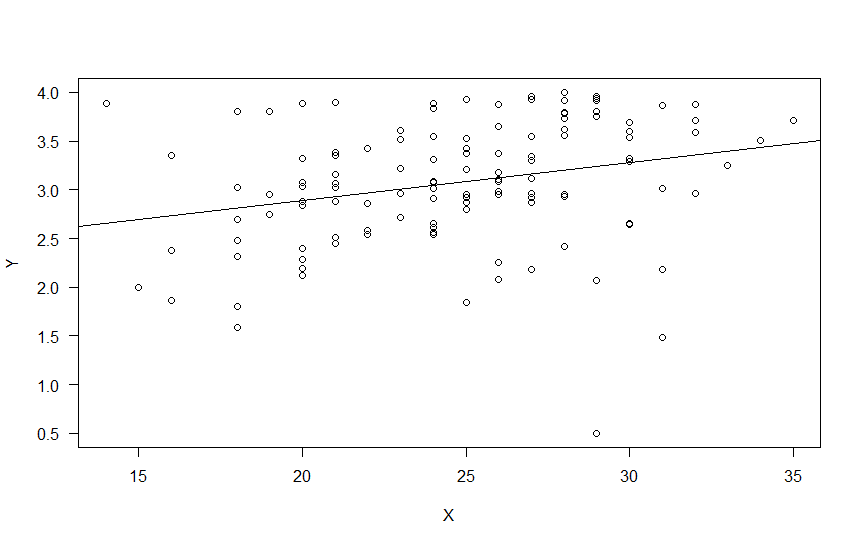
\includegraphics[width=0.90\textwidth]{Rplot01.png}

Surely it doesn't fit the data very well.

\subsubsection{c.}
With $X=30$, we can obtain that $\hat{Y}=\beta_0+\beta_1 X=3.278863$

\subsubsection{d.}
Let $\delta$ be the change,$$\hat{\delta}=\beta_1=0.03883$$

\subsection{3.}
\subsubsection{a.}
From $\hat{\beta_1}=argmin_{\beta_1}Q$, where $Q=\sum_{i=1}^n(Y_i-\beta_1X_i)^2$, we obtain:

$$\frac{\partial Q}{\partial\beta_1}=-2\sum_{i=1}^nX_i(Y_i-\beta_1X_i)=0$$

It can be solved:

$$\hat{\beta_1}=\frac{\sum_{i=1}^nX_iY_i}{\sum_{i=1}^nX_i^2}$$

\subsubsection{b.}
\begin{align*}
    &\because \epsilon_i=Y_i-\beta_1X_i\ i.i.d.\sim N(0,\sigma^2)\\
    &\begin{aligned}
        \therefore L(\beta_1|X_1,\cdots,X_n,Y_1,\cdots,Y_n)&=(2\pi\sigma^2)^{-n/2}exp(-\frac{\sum_{i=1}^n\epsilon_i^2}{2\sigma^2})\\
        &=(2\pi\sigma^2)^{-n/2}exp(-\frac{\sum_{i=1}^n(Y_i-\beta_1X_i)^2}{2\sigma^2})
    \end{aligned}\\
    &\therefore logL=-\frac{n}{2}log(2\pi\sigma^2)-\frac{\sum_{i=1}^n(Y_i-\beta_1X_i)^2}{2\sigma^2}\\
    &\text{From}\frac{\partial logL}{\partial \beta_1}=0 \text{ It can be solved:}\\
    &\hat{\beta_1}=\frac{\sum_{i=1}^nX_iY_i}{\sum_{i=1}^nX_i^2},\text{ the same as the LSE.}
\end{align*}

\subsubsection{c.}
\begin{align*}
    &
    \begin{aligned}
        \because E\hat{\beta_1}&=\frac{1}{\sum_{i=1}^nX_i^2}E\sum_{i=1}^nX_iY_i\\
        &=\frac{1}{\sum_{i=1}^nX_i^2}E(\beta_1X_i^2+X_i\epsilon_i)\\
        &=\beta_1+\frac{\sum_{i=1}^nX_iE\epsilon_i}{\sum_{i=1}^nX_i^2}\\
        &=\beta_1
    \end{aligned}\\
    &\therefore \hat{\beta_1}\text{ is unbiased.}
\end{align*}

\subsection{4.}
\subsubsection{a.}
Denote $X_i$ as the i-th recovery time, $s^2=\frac{1}{n-1}\sum_{i=1}^n(X_i-\bar{X})^2$.

Consider $X_i\ i.i.d.\sim N(\mu,\sigma^2)$,$\bar{X}\sim N(\mu,\sigma^2/n)$

$$H_0: \mu=123.7\leftrightarrow H_1:\mu>123.7$$

$$\text{Let }T=\frac{\sqrt{n}(\bar{X}-123.7)}{s}\sim t_{n-1}$$

From $P(T>t_{n-1;0.1})=10\%$ we can decide to reject $H_0$ if $T>t_{n-1;0.1}$.

Because $T=2.0687>t_{6;0.1}$, we don't reject $H_0$


\subsubsection{b.}
The same as a, because $T=2.0687>t_{6;0.05}$

\subsection{5.}
From what we have proved we can obtain:

\begin{align*}
    b_0&=\bar{Y}-b_1\bar{X}\\
    &=\bar{Y}-\beta_1\bar{X}-\frac{\sum(X_i-\bar{X})\epsilon_i}{\sum(X_i-\bar{X})^2}\bar{X}\\
    &=\beta_0+\frac{\sum\epsilon_i}{n}-\frac{\sum(X_i-\bar{X})\epsilon_i}{\sum(X_i-\bar{X})^2}\bar{X}\\
\end{align*}

\begin{align*}
    &\because E(b_0)=E(\bar{Y}-\beta_1\bar{X})+0=E(\frac{\sum(\beta_0+\epsilon_i)}{n})=\beta_0\\
    &\therefore b_0\text{ is unbiased.}\\
    &\because Var(b_0)=\sum(\frac{1}{n}-\frac{\bar{X}\sum(X_i-X)}{\sum(X_i-X)^2})^2\sigma^2\\
\end{align*}

\subsection{6.}
\begin{align*}
    &
    \begin{aligned}
        \because Q&=\sum(Y_i-b_0-b_1X_i)^2\\
        &=\sum((\beta_0-b_0)+(\beta_1-b_1)X_i)^2\\
        &=\sum_i(\sum_j\epsilon_j(\frac{1}{n}+\frac{(X_j-\bar{X})(X_i-\bar{X})}{\sum_k(X_k-\bar{X})^2}))^2\\
    \end{aligned}\\
    &\therefore E(Q)=(n-2)(E\epsilon_i^2-(E\epsilon)^2)=(n-2)Var(\epsilon)=(n-2)\sigma^2
\end{align*}
\end{document}